\subsection{Ethereum}
\label{subsec:ethereum}

Ethereum adalah sebuah platform berbasis Blockchain untuk membangun aplikasi terdesentralisasi dan Smart Contracts, dengan serangkaian \textit{tradeoffs} yang berbeda. Dikembangkan oleh Vitalik Buterin pada tahun 2015, Ethereum mengembangkan konsep dasar Blockchain dengan menambahkan sebuah bahasa pemrograman \textit{Turing-complete} untuk mengembangkan Smart Contracts, yang dijalankan di dalam Ethereum Virtual Machine (EVM). Ethereum Virtual Machine (EVM) adalah sebuah lingkungan eksekusi untuk Smart Contracts di Ethereum, yang memungkinkan kode berjalan di seluruh jaringan Ethereum secara terdistribusi. Bahasa pemrograman bawaan Ethereum yang \textit{Turing-complete} adalah Solidity, yang digunakan untuk menulis Smart Contracts di Ethereum. Solidity adalah bahasa dengan paradigma berorientasi objek, seluruh program Smart Contract akan dikompilasi menjadi sebuah \textit{byte-code}, dalam kasus ini menjadi bentuk EVM Bytecode, dan spesifikasinya dituliskan pada sebuah Application Binary Interface (ABI). Dengan bahasa pemrograman yang \textit{Turing-complete} dan mekanisme eksekusi yang terjamin dengan EVM, Ethereum memberikan kemampuan bagi pengembang untuk mengembangkan sebuah aplikasi yang terdesentralisasi, yang disebut juga sebagai \textit{dApps}, dimana kode dan data disimpan di dalam Blockchain, sehingga mendapatkan karakteristik bawaan dari karakteristik Blockchain \parencite{buterin2013ethereum}.

\subsubsection{ABI}
\label{subsubsec:abi}

\begin{figure}[ht]
  \centering
  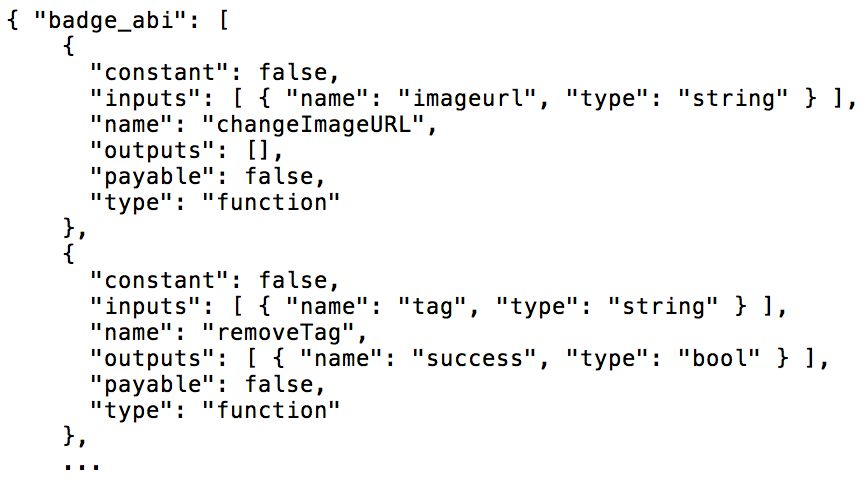
\includegraphics[width=0.7\textwidth]{resources/chapter-2/smart-contract-abi.jpg}
  \caption{Contoh ABI dari sebuah Smart Contract \parencite{third2017linked}}
  \label{image:abi-example}
\end{figure}

Application Binary Interface (ABI) adalah sebuah konvensi yang mendefinisikan aspek-aspek kode yang dihasilkan selama kompilasi, seperti representasi data, penggunaan register, dan konvensi pemanggilan fungsi \parencite{sciencedirect2024}. Dalam konteks Smart Contracts yang ditulis dengan bahasa Solidity dan dikompilasi, hasil dari kompilasinya akan berbentuk EVM Bytecode untuk dieksekusi di dalam EVM, disertai dengan ABI yang mendefinisikan Smart Contract tersebut, seperti pada gambar \ref{image:abi-example}.

\subsubsection{Etherscan}
\label{subsubsec:etherscan}

Etherscan adalah \textit{block explorer}, sebuah \textit{search engine} agar pengguna dapat dengan mudah melihat, mengonfirmasi, dan memvalidasi transaksi untuk Blockchain Ethereum. Etherscan berdiri secara independen dari Ethereum Foundation, yang melakukan \textit{indexing} terhadap Blockchain untuk menampilkan informasinya \parencite{etherscan2024}.